\subsection{Nixtla Neural Forecast TimeGPT}
{{\footnotesize
\noindent TimeGPT is a transformer-based generative pretrained model on 100B+ time series data for
zero-shot forecasting and anomaly detection via API .


\begin{description}[labelwidth=4cm, labelsep=1em, leftmargin=4cm, itemsep=0.1em, parsep=0em]
  \item[date:] 2023-10-05
  \item[version:] v3.0.2
  \item[last\_updated:] 2025-06
  \item[expired:] unknown
  \item[valid:] yes
  \item[valid\_date:] 2023-10-05
  \item[url:] \href{https://github.com/Nixtla/neuralforecast}{https://github.com/Nixtla/neuralforecast}
  \item[doi:] 10.48550/arXiv.2310.03589
  \item[domain:] Time-series; General ML
  \item[focus:] Time-series foundation model "TimeGPT" for forecasting and anomaly detection
  \item[keywords:]
    - TimeGPT
    - foundation model
    - time-series
    - generative model
  \item[licensing:] Apache License 2.0
  \item[task\_types:]
    - Time-series forecasting
    - Anomaly detection
  \item[ai\_capability\_measured:]
    - Zero-shot forecasting
    - anomaly detection
  \item[metrics:]
    - RMSE
    - Anomaly detection metrics
  \item[models:]
    - TimeGPT
  \item[ml\_motif:]
    - Time-series
  \item[type:] Platform
  \item[ml\_task:]
    - Forecasting
  \item[solutions:] Solution details are described in the referenced paper or repository.
  \item[notes:] Offered via Nixtla API and Azure Studio; enterprise-grade support available.

  \item[contact.name:] Azul Garza (Nixtla)
  \item[contact.email:] unknown
  \item[results.links.name:] ChatGPT LLM
  \item[fair.reproducible:] Yes
  \item[fair.benchmark\_ready:] Yes
  \item[id:] nixtla\_neural\_forecast\_timegpt
  \item[Citations:] \cite{garza2024timegpt1}
\end{description}

{\bf Ratings:} ~ \\

\begin{tabular}{p{0.15\textwidth} p{0.07\textwidth} p{0.7\textwidth}}
\hline
Rating & Value & Reason \\
\hline
dataset & 3 & Evaluated on existing open datasets, but consolidated data release, splits, and FAIR
metadata are not provided.
 \\
documentation & 3 & Basic README with installation and usage examples; more detailed API docs and tutorials
would improve usability.
 \\
metrics & 4 & Uses standard forecasting metrics such as RMSE, MASE, SMAPE, and anomaly detection
metrics consistently across evaluations.
 \\
reference\_solution & 3 & TimeGPT implementation is available, but baseline comparisons and additional reference
models are limited.
 \\
software & 4 & Fully open-source Apache 2.0 implementation integrated in NeuralForecast,
supporting training and evaluation via API. Production-grade deployment available via Nixtla API and Azure.
 \\
specification & 3 & Concept and forecasting goals are described, but formal input/output definitions
and task constraints are not rigorously specified.
 \\
\hline
\end{tabular}

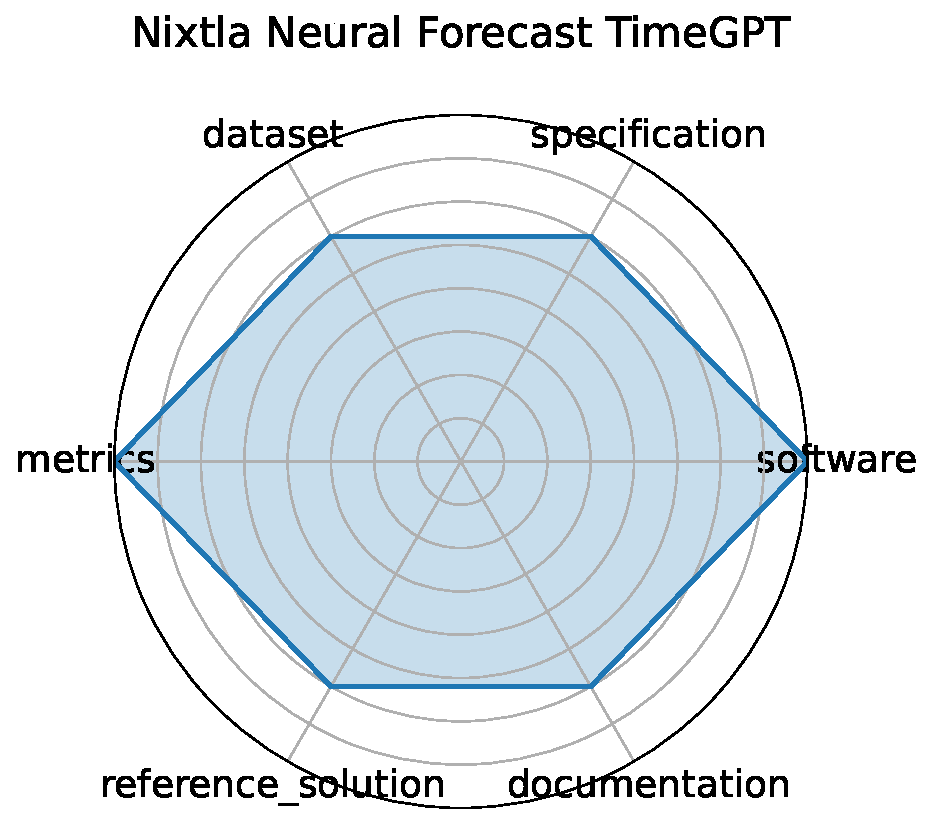
\includegraphics[width=0.2\textwidth]{nixtla_neural_forecast_timegpt_radar.pdf}
}}
\clearpage